%\section{Smartphone}%
%\label{sec:smartphone-design}
The smartphone design was divided into three stages, the functional model, the object model and the dynamic model.

\subsection{Functional Model}
The functional model includes a description of the system in terms of accessible functionalities from the actors' point of view, represented in figure \ref{fig:usecase_android}.
%
In this stage, the actors identified were the user, the \gls{nvs} and the \gls{rvvs}. The user must have access to three key features:
% 
\begin{itemize}%
\item \textbf {Vehicle control}: the ability to control the car by tilting the smartphone and thereby changing the provided angle and speed reference. This feature implies a transmission of these values to the \gls{nvs} and a UI value update.
\item \textbf {Notification view}: pop-ups that allow a grasp of the current state of the system with informative or alert messages.
\item \textbf {Video feed view}: Be able to visualize the \gls{rvvs}` video transmission on screen.
\end{itemize}
%
On one hand, the \gls{nvs} should be able to receive the accelerometer data provided while also sending notifications to the app, both via Bluetooth.
%
On the other hand, the \gls{rvvs} should be capable of transmitting the camera´s video while also sending the same type of notifications to the user within the application. This communication is established via Wifi/GPRS.
%
\begin{figure}[!ht]
\centering
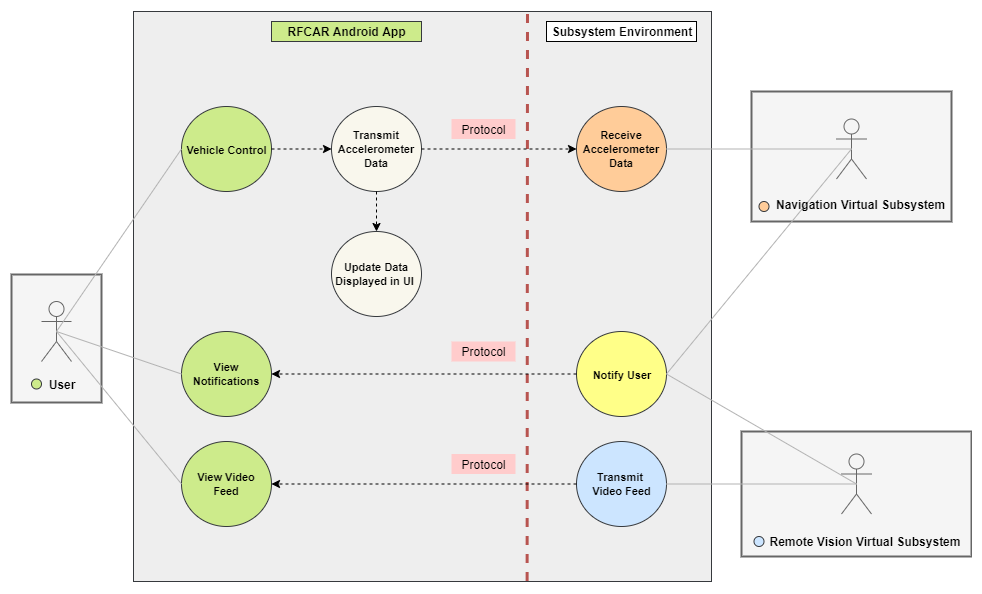
\includegraphics[width=0.8\textwidth]{img/UseCaseAndroid.png}
\caption{\label{fig:usecase_android}Android app use case diagram.}
\end{figure}
%
\subsection{Object/Static Model}
In this step, the objective was to define the app system´s structure with \gls{uml} class diagrams, concerning its objects, attributes, operations and associations established.  The first, of the forementioned diagrams, is represented in figure \ref{fig:uml-android}.
%
\begin{figure}[!ht]
\centering
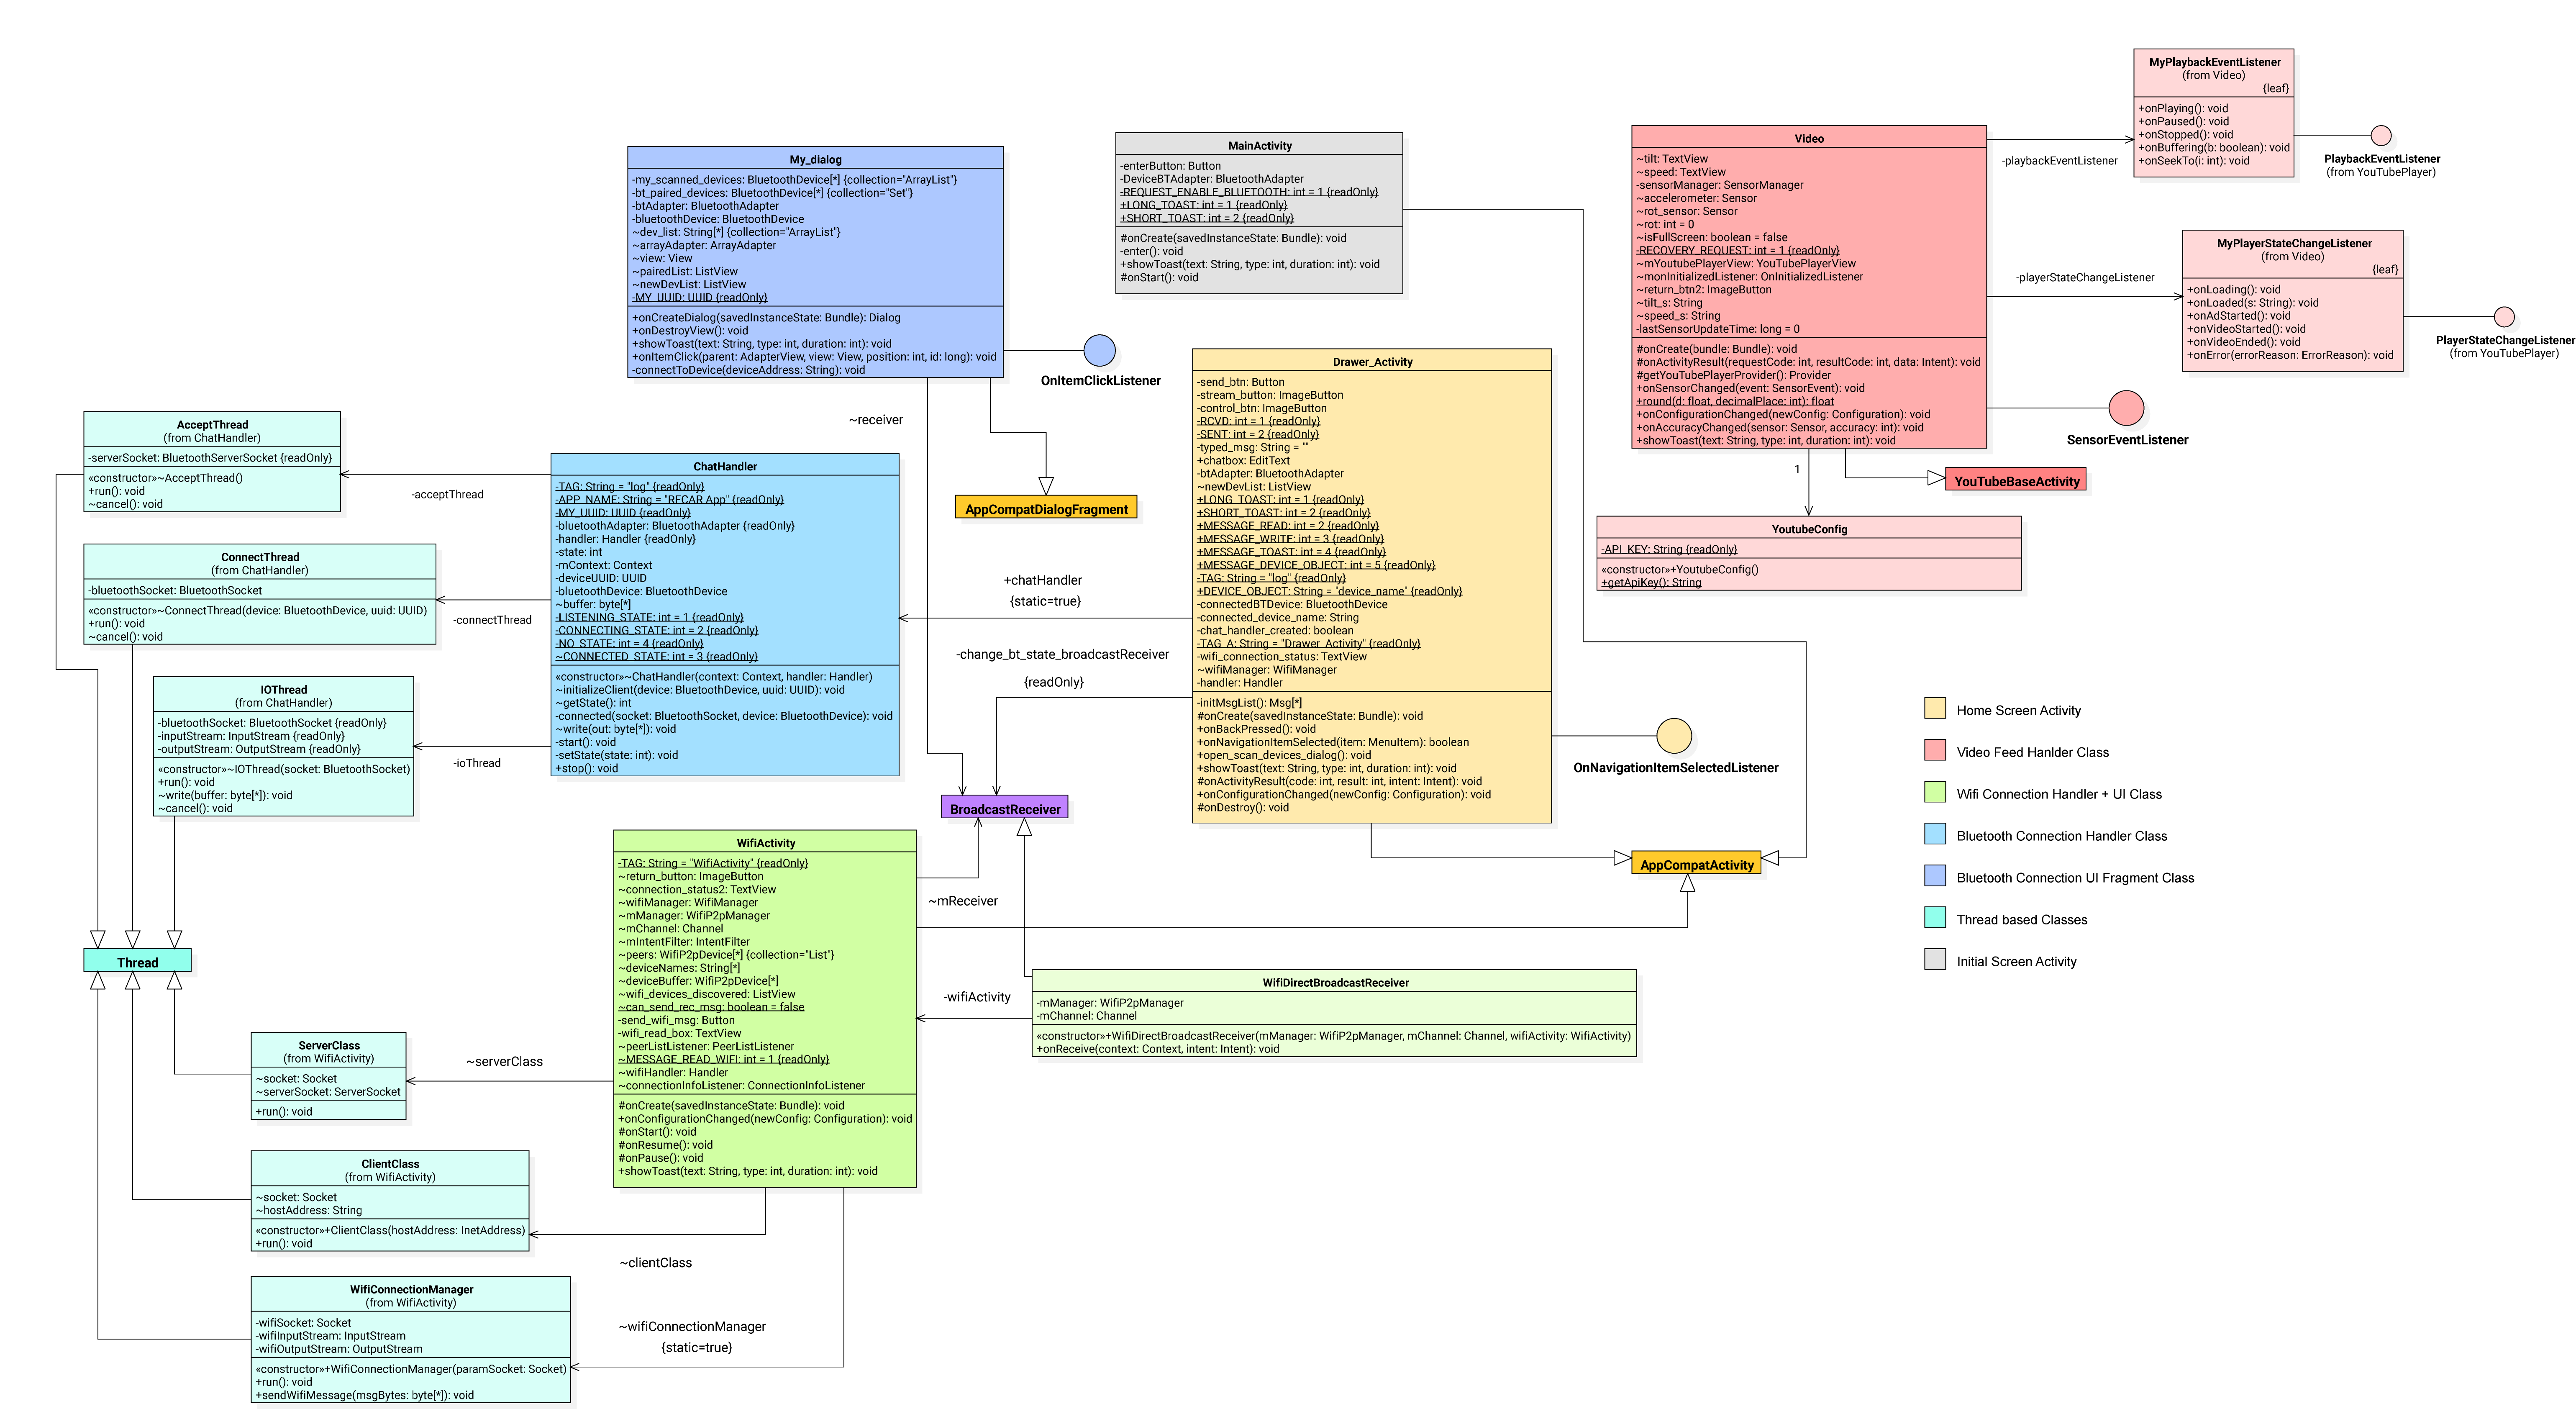
\includegraphics[width=\textwidth]{img/smartphone-static-diagram.png}
\caption{\label{fig:uml-android}Smartphone class diagram}
\end{figure}
%
\subsection{Dynamic Model}
For the dynamic model, were devised multiple state-machine diagrams to describe the internal behaviour of the application. 
%
Figure \ref{fig:overall_system_diagram} illustrates the overall application behaviour. One can observe that all the intended features are meant to run in parallel, that will surely affect the system implementation in terms of concurrency (section \ref{sec:concurrency}) and thread management.
%
Initially, the system loads the \gls{ui} and waits for all connections to be established before moving to the next state.
%
While the feature for vehicle control is running (figure \ref{fig:vehicle_control_diagram}) it retrieves the accelerometer data, sends the data to the \gls{nvs} and displays it on the screen.
%
Additionally, the feature that allows the user to see the video feed transmitted by the \gls{rvvs} in figure \ref{fig:video_feed_diagram} also displays it on the app screen. When this Wifi/GPRS connection is suspended by any means, it should exist an immediate reconnection to the \gls{rvvs}.
%
The notifications presented to the user should indicate the current state of the system, which means displaying informative messages, like successful connections but also alert messages like the ones displayed in figure \ref{fig:notification_diagram}.
%
\begin{figure}[!ht]
\centering
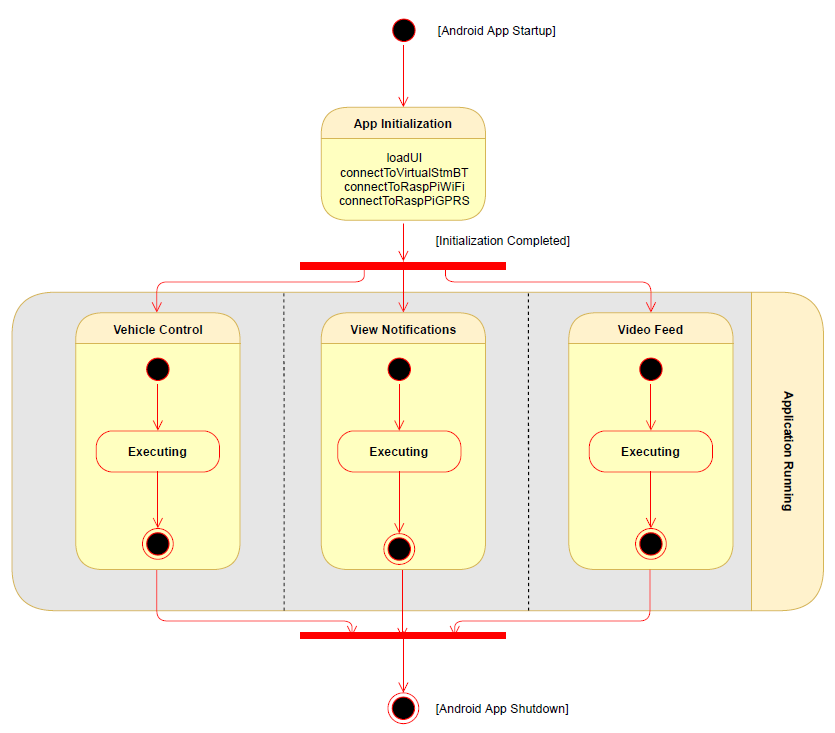
\includegraphics[width=0.7\textwidth]{img/overall_system_sm.png}
\caption{\label{fig:overall_system_diagram}Overall system behaviour diagram.}
\end{figure}
%
\begin{figure}[!ht]
\centering
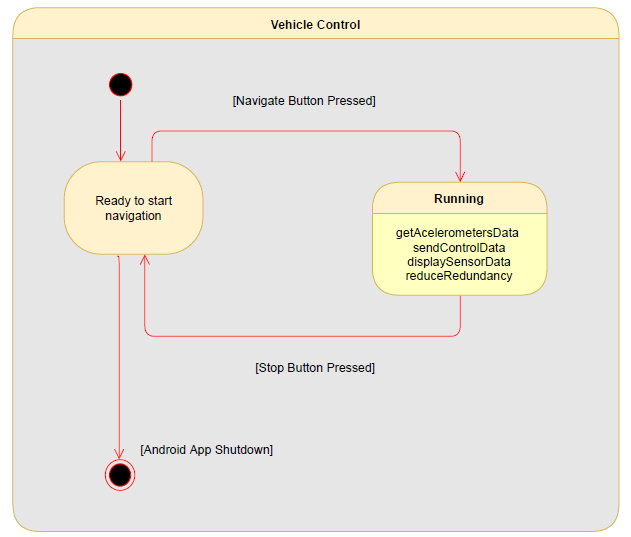
\includegraphics[width=0.7\textwidth]{img/vehicle_control_sm.png}
\caption{\label{fig:vehicle_control_diagram}Vehicle control feature diagram.}
\end{figure}
%
\begin{figure}[!ht]
\centering
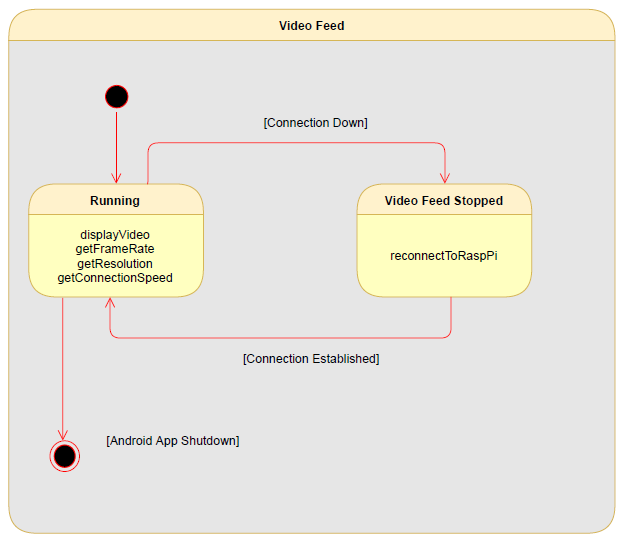
\includegraphics[width=0.7\textwidth]{img/video_feed_sm.png}
\caption{\label{fig:video_feed_diagram}Video feed feature diagram.}
\end{figure}
%
\begin{figure}[!ht]
\centering
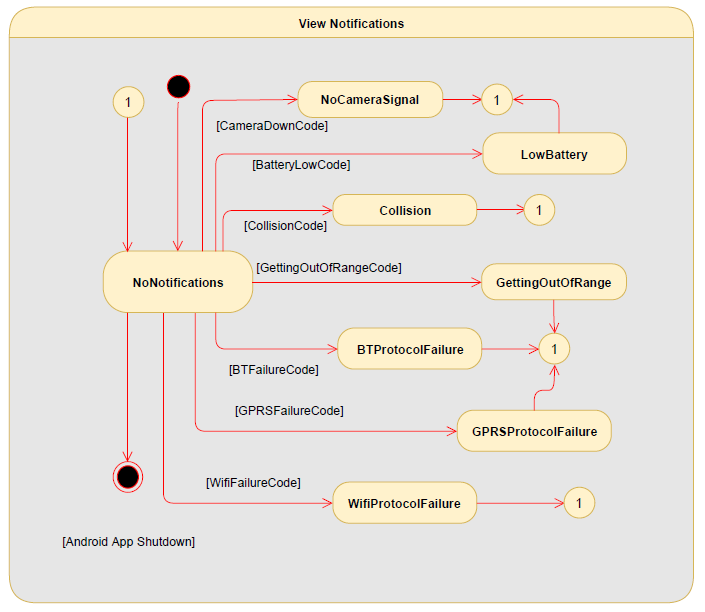
\includegraphics[width=0.7\textwidth]{img/notification_sm.png}
\caption{\label{fig:notification_diagram}Notification feature diagram.}
\end{figure}
%